\subsection{Diseño de la Zona de Recolección}

La zona de recolección constituye el área donde se posicionan los objetos a clasificar antes de su manipulación por el robot. Su diseño se fundamentó en criterios de accesibilidad robótica, optimización para visión por computador y aprovechamiento del espacio disponible en la plataforma.

\subsubsection{Configuración Geométrica y Ubicación}

El área de recolección se definió a partir del espacio disponible en el layout una vez posicionados la base del manipulador y las cuatro zonas de depósito. Como se observa en el layout de la Figura \ref{fig:layout2}, la zona de recolección ocupa el área circular central delimitada por estos componentes.

La ubicación centrada en la plataforma base ofrece ventajas significativas:

\begin{itemize}
    \item \textbf{Optimización del campo visual}: La posición central respecto a la cámara superior facilita la captura de imágenes con iluminación uniforme y mínima distorsión perspectiva
    \item \textbf{Accesibilidad robótica}: Todos los puntos de la zona de recolección se encuentran dentro del alcance efectivo del manipulador sin requerir configuraciones extremas
    \item \textbf{Simetría operativa}: La distribución equidistante respecto a las cuatro zonas de depósito simplifica la planificación de trayectorias
\end{itemize}

\begin{figure}[H]
    \centering
    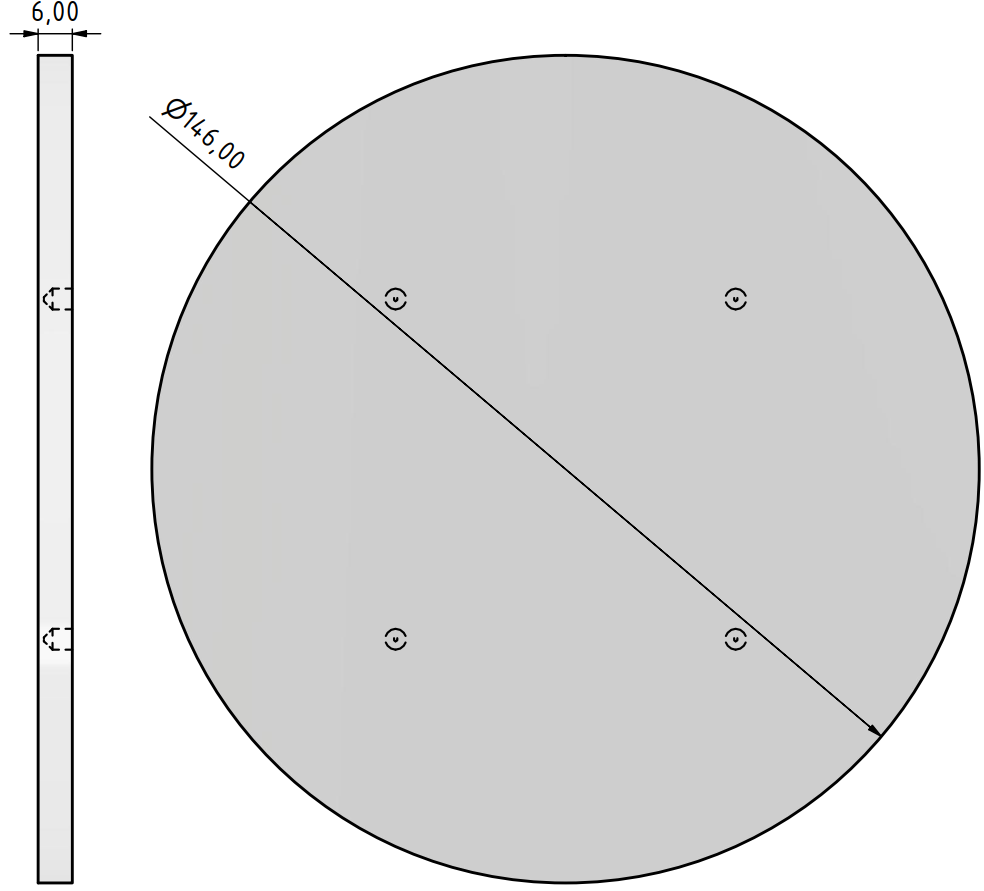
\includegraphics[width=0.6\textwidth]{06disenoConceptual/img/zonaRecoleccion/zonaRecoleccionRedonda.png}
    \caption{Vista superior de la zona de recolección con dimensiones principales. Diámetro exterior: Ø146 mm. Altura: 6 mm mínimo (determinado por el alojamiento de insertos roscados M3 en la cara inferior). Se observan cuatro agujeros ciegos para instalación de insertos roscados distribuidos simétricamente.}
    \label{fig:zonaRecoleccionRedonda}
\end{figure}

\subsubsection{Selección de Color y Acabado Superficial}

Se seleccionó el color blanco para la superficie de la zona de recolección por razones relacionadas con el desempeño de los algoritmos de visión por computador:

\begin{enumerate}
    \item \textbf{Máximo contraste con objetos}: La superficie blanca proporciona contraste elevado con objetos de colores típicamente utilizados en tareas de clasificación (rojo, verde, azul, amarillo, negro)
    
    \item \textbf{Balance de blancos}: Facilita la calibración automática del balance de blancos de la cámara, mejorando la reproducción cromática de los objetos
    
    \item \textbf{Iluminación difusa}: La superficie blanca refleja luz de manera más uniforme que colores oscuros, reduciendo sombras pronunciadas que puedan interferir con la segmentación de objetos
    
    \item \textbf{Contraste con plataforma base}: La zona blanca sobre la plataforma base negra crea una delimitación visual clara del área de trabajo
\end{enumerate}

\subsubsection{Sistema de Fijación}

La zona de recolección se fija a la plataforma base mediante cuatro insertos roscados M3 para plástico instalados en la cara inferior. Este sistema proporciona múltiples ventajas:

\begin{itemize}
    \item \textbf{Superficie superior limpia}: Al ubicarse los insertos y tornillos en la cara inferior, la superficie superior queda completamente libre de elementos de fijación visibles, eliminando potenciales interferencias con los algoritmos de visión
    
    \item \textbf{Simplificación visual}: La zona de recolección se presenta como una superficie circular blanca uniforme, facilitando su identificación automática y la detección de objetos sobre ella
    
    \item \textbf{Restricción de altura mínima}: Los insertos roscados M3 requieren una profundidad de alojamiento que establece una altura mínima de 6 mm para la zona de recolección, valor que resulta adecuado para proporcionar un pequeño escalón que delimita visualmente el área
\end{itemize}

\subsubsection{Ensamble del Conjunto}

El conjunto completo de la zona de recolección se presenta en la Figura \ref{fig:ensambleZonaRecoleccion}.

\begin{figure}[H]
    \centering
    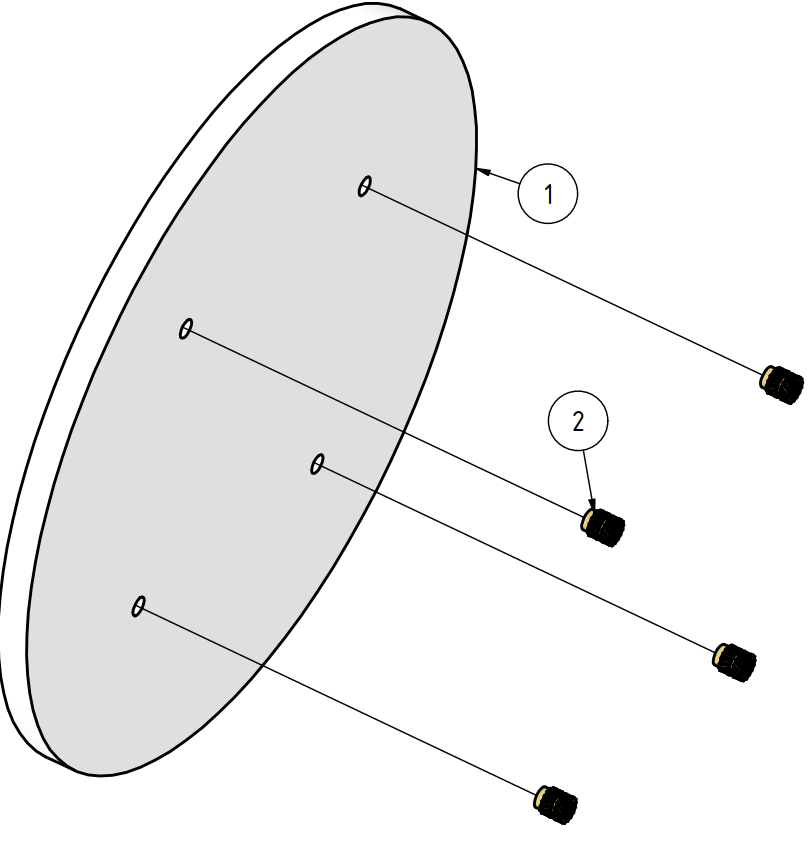
\includegraphics[width=0.55\textwidth]{06disenoConceptual/img/zonaRecoleccion/ensambleZonaRecoleccion.png}
    \caption{Ensamble explosionado de la zona de recolección. (1) Disco circular fabricado mediante FDM en filamento blanco (PLA o ABS), (2) Tornillos M3 × 15 mm que atraviesan la plataforma base y se enroscan en los insertos roscados ubicados en la cara inferior del disco.}
    \label{fig:ensambleZonaRecoleccion}
\end{figure}

\begin{table}[H]
\centering
\caption{Lista de materiales de la zona de recolección}
\label{tab:bom_zona_recoleccion}
\small
\begin{tabular}{|c|l|c|l|l|}
\hline
\textbf{\#} & \textbf{Componente} & \textbf{Cant.} & \textbf{Fabricación} & \textbf{Material} \\
\hline
1 & Zona de recolección & 1 & FDM & PLA/ABS blanco \\
2 & Inserto roscado M3 & 4 & Comercial & Latón \\
3 & Tornillo M3 × 15 mm & 4 & Comercial & Acero \\
\hline
\end{tabular}
\end{table}

La simplicidad de este diseño contrasta favorablemente con la complejidad de las canecas de la primera iteración, demostrando que la funcionalidad óptima no siempre requiere soluciones elaboradas. La zona de recolección cumple eficientemente su propósito mediante una geometría simple, un sistema de fijación robusto y una selección de color fundamentada en principios de visión por computador.